\chapter{Funzionalità dell'applicazione}

Come detto durante l'analisi della struttura del progetto, la nostra applicazione è strutturata 
    con due classi principali: \texttt{MainActivity} e \texttt{PdfActivity}. 
    Questo ci permette di distinguere e separare le due funzionalità principali della nostra applicazione.\\
    \\
    \noindent Nell'immagine sotto, viene mostrata la HomePage della nostra applicazione, dotata di soli due pulsanti.

\begin{figure}[H]
    \centering
    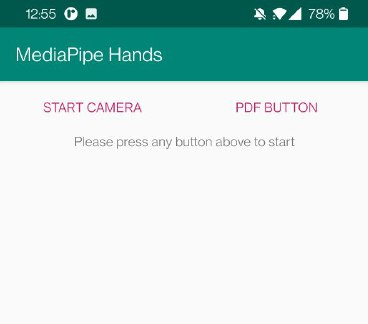
\includegraphics[width=0.5\textwidth]{images/homepage.png}
\end{figure}



\newpage
\section{MainActivity}

\begin{multicols}{2}
\noindent Questa classe corrisponde all'entry point della nostra applicazione. All'interno di essa sono stati definiti due pulsanti: \texttt{StartCamera} e \texttt{PdfButton}.\\
Il primo permette di attivare la telecamera frontale 
del nostro dispositivo Android, previa autorizzazione dell'utente.\\
\\
\noindent In questo caso viene mostrato lo 
stream della videocamera in tempo reale, elaborato quasi istantaneamente dalle nostre 
implementazioni, in modo da ridurre il ritardo che ne potrebbe scaturire e dunque uno sfasamento 
temporale che porterebbe al lag della nostra applicazione.
    \columnbreak
    \begin{multicolfigure}
        \centering
        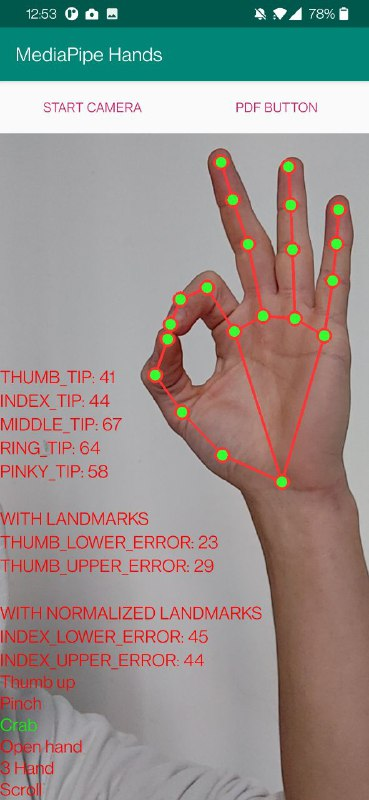
\includegraphics[width=0.9\textwidth]{images/startcamera.png}
    \end{multicolfigure}
\end{multicols}

\noindent In questo scenario, attivando la videocamera, verrà presentato all'utente l'immagine della fotocamera interna con la sua mano mappata da 21 punti 
differenti (\textit{landmarks}), ovvero 4 punti per dito, che ci permettono di differenziare le varie falangi, e un punto per 
il polso che ci permette di riconoscere l'orientamento della mano e la profonfità relativa.\\
\\
\noindent Abbiamo utilizzato questa funzionalità per sperimentare le varie gesture da noi implementate, osservando nelle \texttt{TextView} da noi create
l'effettivo cambiamento delle coordinate dei punti che identificano le nostre dita, nonché il 
riconoscimento della gesture eseguita, la cui scritta verrà colorata di verde (rossa in origine).


\newpage
\section{PdfActivity}
Dopo aver testato e dimostrato il corretto funzionamento del nostro applicativo, abbiamo deciso di applicare 
    quanto appena appreso a contesti quotidiani in modo da renderlo utile e funzionale per eventuali 
    utilizzatori. Abbiamo dunque applicato le nostre gesture alla lettura e all'interazione con un file pdf.
\begin{multicols}{2}
    \noindent Cliccando infatti sul quarto ed ultimo bottone della \texttt{MainActivity}, ovvero \textit{"Pdf Button"}, andiamo 
    tramite un \texttt{Intent} a creare una nuova schermata, chiamata \texttt{PdfActivity}, che svolge le funzionalità 
    appena espresse.\\
    \\
    \noindent In questa schermata abbiamo creato 2 View separate: una, la principale, per 
    mostrare il pdf (effettuato utilizzando un \texttt{PdfViewer} ottenuto grazie alla libreria esterna 
    \texttt{com.github.mhiew}), l'altra, di dimensioni ridotte e posta sopraelevata in basso a destra, per 
    gestire la videocamera frontale e per consentire, dunque, all'utente, di vedere le gesture 
    effettuate.
        \columnbreak
        \begin{multicolfigure}
            \centering
            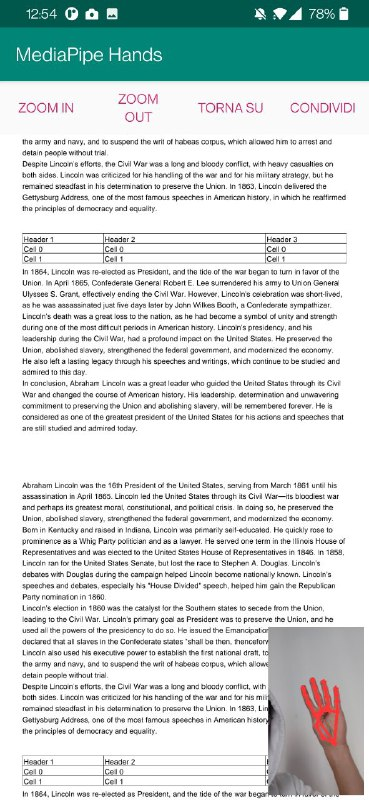
\includegraphics[width=0.8\textwidth]{images/pdfactivity.png}
        \end{multicolfigure}
    \end{multicols}


\newpage
\subsection{Mapping delle gesture con azioni del pdf}
Abbiamo così applicato il lavoro effettuato nel nostro MainActivty al pdf, mappando le gesture definite in precedenza a determinati azioni sul file pdf.

\begin{itemize}
    \item Gesture statiche \begin{itemize}
        \item \textbf{Thumb up}: apertura del prompt di condivisone del pdf mostrato.
        \item \textbf{Three hand}: comparsa di un \texttt{AlertDialog} per la scelta del pdf da visualizzare (creati una sola volta al primo avvio tramite la libreria \texttt{iTextPdf} e poi mantenuti in memoria).
        \item \textbf{Four hand}: scroll continuo verticale del pdf, che scende di 40 pixel al secondo, in modo da emulare la lettura del file stesso.
    \end{itemize}
    \item Gesture dinamiche \begin{itemize}
        \item \textbf{Crab}: rende possibile muoversi all'interno del pdf (scroll) in qualsiasi direzione.
        \item \textbf{Pinch}: si incrementa o diminuisce il valore dello zoom sul pdf aumentando o riducendo la distanza tra indice e pollice.
        \item \textbf{Scroll}: permette di cambiare pagina verso sinistra o verso destra, in base alla direzione del movimento.
    \end{itemize}
    
\end{itemize}

